\subsection{O Método Van Albada}

O limitador de Van Albada é amplamente utilizado em métodos TVD devido à sua capacidade de reduzir oscilações artificiais enquanto mantém a suavidade das soluções numéricas. O limitador é dado por:

\begin{equation}
    \phi(\theta) = \frac{\theta + \theta^2}{1 + \theta^2 + \epsilon},
\end{equation}

onde \(\theta\) é o gradiente relativo entre células adjacentes, e \(\epsilon\) é um pequeno valor para evitar divisões por zero.

\begin{figure}[H]
    \centering
    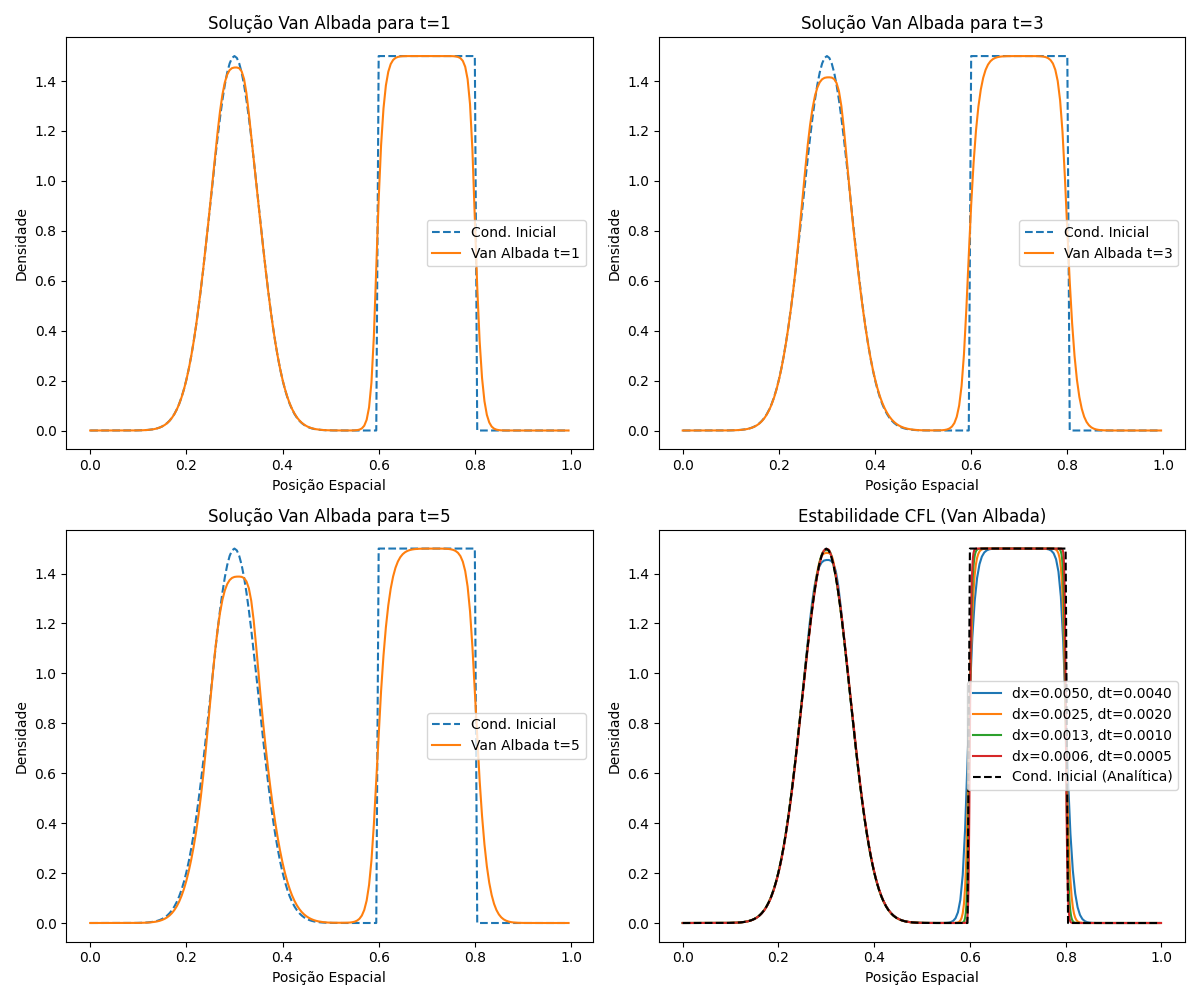
\includegraphics[width=\textwidth]{code/images/Van Albada.png}
    \caption{Solução Van Albada para \( t=1 \), \( t=3 \), e \( t=5 \), com a condição inicial representada pela linha tracejada.}
\end{figure}

\begin{table}[H]
    \centering
    \begin{tabular}{rrrrrr}
\toprule
Posicao Espacial & Condicao Inicial & Van Albada t=1 & Van Albada t=3 & Van Albada t=5 & Posicao da Estabilidade \\
\midrule
0.000000 & 0.000000 & 0.000000 & 0.000001 & 0.000002 & 0.000000 \\
0.050000 & 0.000006 & 0.000007 & 0.000010 & 0.000010 & 0.050000 \\
0.100000 & 0.000503 & 0.000508 & 0.000518 & 0.000385 & 0.100000 \\
0.150000 & 0.016663 & 0.016514 & 0.016224 & 0.012514 & 0.150000 \\
0.200000 & 0.203003 & 0.202423 & 0.201549 & 0.169463 & 0.200000 \\
0.250000 & 0.909796 & 0.913083 & 0.945764 & 0.894611 & 0.250000 \\
0.300000 & 1.500000 & 1.454065 & 1.414557 & 1.386331 & 0.300000 \\
0.350000 & 0.909796 & 0.905613 & 0.905565 & 1.003061 & 0.350000 \\
0.400000 & 0.203003 & 0.204138 & 0.206437 & 0.241922 & 0.400000 \\
0.450000 & 0.016663 & 0.017666 & 0.019614 & 0.026521 & 0.450000 \\
0.500000 & 0.000503 & 0.000601 & 0.000751 & 0.001335 & 0.500000 \\
0.550000 & 0.000006 & 0.000587 & 0.004220 & 0.005270 & 0.550000 \\
0.600000 & 1.500000 & 0.924996 & 0.903320 & 0.759428 & 0.600000 \\
0.650000 & 1.500000 & 1.499387 & 1.492678 & 1.477461 & 0.650000 \\
0.700000 & 1.500000 & 1.500000 & 1.499982 & 1.499808 & 0.700000 \\
0.750000 & 1.500000 & 1.499776 & 1.497832 & 1.497129 & 0.750000 \\
0.800000 & 1.500000 & 0.852868 & 0.798934 & 0.926993 & 0.800000 \\
0.850000 & 0.000000 & 0.001463 & 0.012478 & 0.034401 & 0.850000 \\
0.900000 & 0.000000 & 0.000000 & 0.000027 & 0.000279 & 0.900000 \\
0.950000 & 0.000000 & 0.000000 & 0.000001 & 0.000003 & 0.950000 \\
\bottomrule
\end{tabular}

    \caption{Tabela de resultados para o método Van Albada nas posições espaciais selecionadas e diferentes tempos.}
    \label{tab:van_albada}
\end{table}

\subsection{Análise dos Resultados do Método Van Albada}

O método Van Albada mostra-se eficaz na preservação da monotonicidade das soluções, mesmo em regiões de gradientes acentuados. Na Figura \ref{fig:van_albada}, observa-se que, para \( t = 1 \), o perfil inicial é bem preservado, com leve dissipação nas bordas. Para \( t = 3 \) e \( t = 5 \), a solução mantém a estabilidade sem introduzir oscilações significativas, destacando a eficiência do limitador de Van Albada em contextos onde a suavidade e precisão são essenciais.

\subsection{Implementação em Python}

O código em Python para o método Van Albada utiliza a função principal \texttt{resolverAdveccaoTVD}, que aplica o limitador e calcula a evolução da densidade ao longo do tempo. A implementação do limitador Van Albada é dada por:

\begin{lstlisting}[language=Python, caption={Código para resolver a advecção usando o método Van Albada}, label={lst:codigo_van_albada}]
def limitadorVanAlbada(theta):
    return (theta + theta**2) / (1 + theta**2 + 1e-6)

def metodoTvdVanAlbada(densidade, nt, intervaloTempo, intervaloEspacial, numeroCourant):
    """
    Método TVD para resolver a advecção utilizando o limitador de Van Albada.
    """
    for n in range(nt):
        novaDensidade = densidade.copy()
        for i in range(len(densidade)):
            esquerda = (i - 1) % len(densidade)
            direita = (i + 1) % len(densidade)
            # Calcula o gradiente relativo (theta)
            theta = (densidade[i] - densidade[esquerda]) / (densidade[direita] - densidade[i] + 1e-6)
            # Fluxos para direita e esquerda
            fluxoDireita = densidade[i] + 0.5 * numeroCourant * (1 - numeroCourant) * limitadorVanAlbada(theta) * (densidade[direita] - densidade[i])
            fluxoEsquerda = densidade[esquerda] + 0.5 * numeroCourant * (1 - numeroCourant) * limitadorVanAlbada(theta) * (densidade[i] - densidade[esquerda])
            # Atualiza a densidade
            novaDensidade[i] = densidade[i] - numeroCourant * (fluxoDireita - fluxoEsquerda)
        densidade = novaDensidade.copy()
    return densidade
\end{lstlisting}

Como visto no código \ref{lst:codigo_van_albada}, o limitador Van Albada suaviza as oscilações enquanto preserva a precisão em gradientes suaves. O número de Courant \(C=0,8\) garante a estabilidade da solução numérica em cada passo temporal.
